\documentclass{article}
\usepackage[T1]{fontenc}
\usepackage[utf8]{inputenc}
\usepackage[swedish]{babel}
\usepackage{amsmath, amssymb, mathtools}
\usepackage{tikz}
\usepackage{enumitem}
\usepackage{siunitx}
\usepackage{ifthen}
\usepackage{listings}
\usepackage{siunitx}
\usepackage{booktabs}
\usepackage{afterpage}
\usepackage{graphicx}

\usetikzlibrary{arrows, decorations.markings, calc, shapes.geometric}

\makeatletter
\def\fps@figure{hbtp}
\def\fps@table{hbtp}
\makeatother

\DeclareMathOperator\rowSums{rowSums}
\DeclareMathOperator\Poisson{Poisson}
\DeclareMathOperator\GammaDist{Gamma}
\DeclareMathOperator\length{length}
\DeclareMathOperator\NegBin{Neg-Bin}

\title{First Assignment in MVE550}
\author{Axel Forsman, Jonas Lauri}

\begin{document}
\maketitle

\section{Question 1}
Let $X$ be the daily number of customers, $X \sim \Poisson(\lambda)$.
The shop receives 2, 0, and 1 customers on Monday, Tuesday, and Wednesday,
respectively.
\begin{enumerate}[label=(\alph*)]
	\item With the assumed prior $\GammaDist(3, 4)$ for $\lambda$,
		compute the posterior given the data above.
        Also, given the data, compute the predicted probabilities for getting zero, 1, 2, 3, or
        4 or more customers on Thursday.
    \item Simulate in R, $N = \num{1e6}$ variables $\lambda_1, ..., \lambda_N$ from the $\GammaDist(3, 4)$
        distribution. For each $\lambda_i$ simulate $y_i$ from the $Poisson(\lambda_i)$ distribution,
        and select those $\lambda_i$ with a simulated $y_i$ value equal to 2.
        Compute theoretically the expected proportion you would select, and
        check with your simulations. Compute also theoretically the distribution
        of the $\lambda_i$ you would select, and compare with the results of
        your simulation.
    \item Starting with the sample above of size one million, simulate for each
        $\lambda_i$ values $y_{i1}, y_{i2}$ and $y_{i3}$ that are $\Poisson(\lambda_i)$ distributed. 
        By comparing the simulated values to 2, 0, and 1, respectively, obtain a
        sample which can be used to obtain an approximate answer to the
        question you answered in (a). Compare your approximate answer to
        your answer from (a).
    \item The answer in (a) can also be computed using numerical integration,
        similar to the example in Section 1.6 of the Lecture Notes. Make
        such a computation, and compare with your results from (a).
\end{enumerate}

\subsection{Part (a)}
Due to the Poisson/Gamma conjugacy, the posterior becomes
\begin{equation*}
    \pi(\lambda \mid X) \sim \GammaDist(\underbrace{3 + \sum_x x}_{=6 \, \eqqcolon \alpha_1},
		\underbrace{4 + \sum_x 1}_{=7 \, \eqqcolon \beta_1}) = \GammaDist(6, 7)
\end{equation*}
If $Y$ is our prediction, where $X$ and $Y$ are iid.,
we get for the distribution of $Y$, again because of the conjugacy,
$\pi(Y \mid X) \sim \NegBin(\alpha_1, \beta_1 / (1 + \beta_1)) = \NegBin(6, 7/8)$.
The predicted probabilites for the different number of customers
are shown in table~\ref{tab:anal_pred_prob}.

\begin{table}
	\caption{Predicted probabilites for different number of customers. \label{tab:anal_pred_prob}}
	\centering
	\begin{tabular}{r r}
		\toprule
		\multicolumn{1}{c}{\bfseries Number of customers, $y$} & \multicolumn{1}{c}{$\mathbb P(Y = y)$} \\
		\midrule
		0 & 0.45 \\
		1 & 0.34 \\
		2 & 0.15 \\
		3 & 0.05 \\
		$\ge 4$ & 0.02 \\
		\bottomrule
	\end{tabular}
\end{table}
\afterpage{\clearpage}

\subsection{Part (b)}
Has the effect of simulating $\mathbb P(Y = 2)$,
where
$$ \Lambda \sim \GammaDist(3, 4), \quad Y \mid \Lambda \sim \Poisson(\lambda) $$
Analytically, through the same argument as above,
the distribution of $Y$ becomes $\NegBin(3, 1 - 1/(1+4))$.
Thus the proportion we expect is $\NegBin(2; 3, 1 - 1/(1+4))$.
Then only picking the $\lambda_i$ for which we have gotten $y_i = 2$
can be compared to taking into account the previous observation $y = 2$.
The distributions are visuallized in figure~\ref{fig:bplot}.
We see that they are very much alike.
The analytical proportion is 0.122880 and the simulated proportion is 0.122819.

\begin{figure}
	\centering
	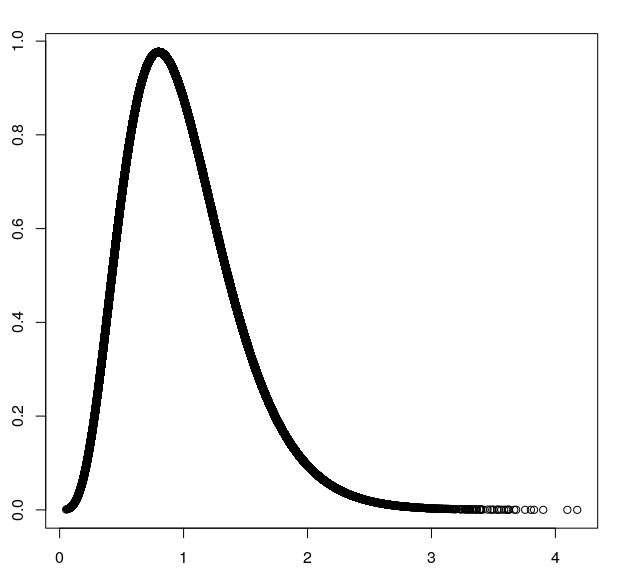
\includegraphics[width=\textwidth]{bplot.png}
	\caption{Plot of simulated and analytical distribution. It's hard to see, but they coincide. \label{fig:bplot}}
\end{figure}
\afterpage{\clearpage}

\subsection{Part (c)}
Following the argument in (b),
we see why the proposed simulation would approximate what we did in (a).
The distributions are visuallized in figure~\ref{fig:cplot}.
We see again that they are very much alike.

\begin{figure}
	\centering
	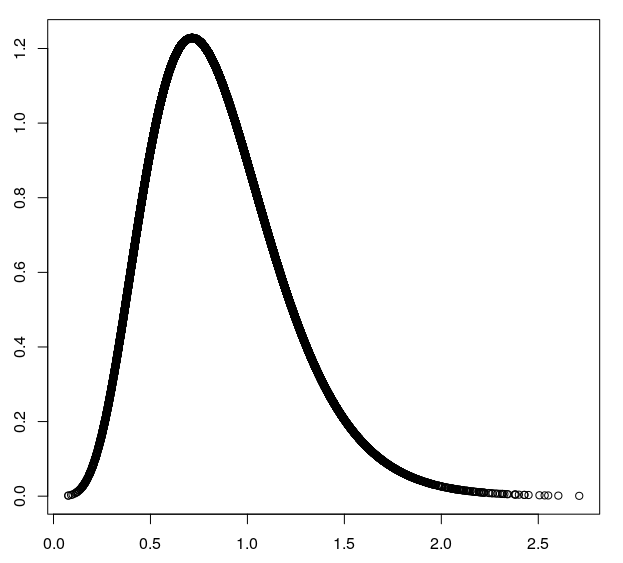
\includegraphics[width=\textwidth]{cplot.png}
	\caption{Plot of simulated and analytical distribution. They coincide. \label{fig:cplot}}
\end{figure}
\afterpage{\clearpage}

\subsection{Part (d)}
Compute $\pi(Y \mid X)$ by numerical integration.
Throwing $\lambda$ into the mix and integrating it out:
\begin{align*}
	\pi(Y \mid X) &= \int_{\Lambda = \mathbb R^+} \pi(Y, \lambda \mid X) \, d\lambda \\
	&= \int_\Lambda \pi(Y \mid X) \pi(\lambda \mid X) \, d\lambda
\end{align*}
where we have used $\pi(Y, \lambda \mid X) = \pi(Y \mid X, \lambda) \pi(\lambda \mid X)$,
and the fact that the prediction given the parameter is independent of the data.
Using Bayes' theorem and the law of total probability
$$ \pi(\lambda \mid X) = \frac{\pi(X \mid \lambda) \pi(\lambda)}{\int_\lambda \pi(X \mid \lambda) \pi(\lambda) \, d\lambda} $$
The calculated probabilites are given in table~\ref{tab:num_pred_prob}. 

\begin{table}
	\caption{Numerically integrated predicted probabilites for different number of customers. \label{tab:num_pred_prob}}
	\centering
	\begin{tabular}{r r}
		\toprule
		\multicolumn{1}{c}{\bfseries Number of customers, $y$} & \multicolumn{1}{c}{$\mathbb P(Y = y)$} \\
		\midrule
		0 & 0.45 \\
		1 & 0.34 \\
		2 & 0.15 \\
		3 & 0.05 \\
		$\ge 4$ & 0.02 \\
		\bottomrule
	\end{tabular}
\end{table}
\afterpage{\clearpage}

\section{Question \num{3.52} in Dobrow.}
With the rule variation that you have to roll the exact number to reach
the final square and that you start on square one.
\begin{enumerate}[label=(\alph*)]
	\item Find the expected length of the game.
	\item Assume that the player is on square 6.
		Find the probability that they will find themselves on square 3 before finishing the game.
\end{enumerate}

\subsection{(a)}

The transition graph is
\begin{center}
	\def\ladderwidth{1.5mm}
	\def\ladderstep{1.5mm}
	\begin{tikzpicture}[
			state/.style={ draw, regular polygon, regular polygon sides=4, fill=gray!15 },
			every edge/.style={ draw, ->,>=stealth', auto, },
			chute/.style={ top color=gray!50, bottom color=gray!50,
			middle color=gray!10, draw=gray!50!black, line cap=round,
			draw opacity=0.3, fill opacity=0.5,
			line join=round,line width=1pt,},
			ladder/.style={decorate,decoration={
				markings,
				mark=between positions {1/#1/2} and {-1/#1/2} step {1/#1} with {
					\draw[draw=gray, draw opacity=0.5,
			line cap=round, line join=round, line width=2pt,]
					(0,-\ladderwidth) -- (0,\ladderwidth)
					(\ladderstep,-\ladderwidth) -- (-\ladderstep,-\ladderwidth)
					(\ladderstep,\ladderwidth) -- (-\ladderstep,\ladderwidth);
					},
					},
					},
					ladder auto/.style={
						to path={
							let \p1=($(\tikztostart) - (\tikztotarget)$), \n1={veclen(\x1,\y1)} in
							\pgfextra{
								\pgfmathsetmacro{\bars}{int(\n1/\ladderstep/2)+1}
								\pgfinterruptpath
								\draw[ladder=\bars] (\tikztostart) -- (\tikztotarget);
								\endpgfinterruptpath
								}
								},
								},
								chute auto/.style={
									to path={
										let
										\p1=([xshift=\ladderwidth]\tikztostart),
										\p2=([xshift=-\ladderwidth]\tikztostart),
										\p3=([xshift=\ladderwidth]\tikztotarget),
										\p4=([xshift=-\ladderwidth]\tikztotarget),
										\p5=($(\p1)!.4!(\p3)$),
										\p6=($(\p2)!.4!(\p4)$)
										in
										\pgfextra{
											\pgfinterruptpath
											\path[chute]
											(\p1) sin (\p5) cos (\p3) --
											(\p4) sin (\p6) cos (\p2) -- cycle;
											\endpgfinterruptpath
											}
											},
											},
											]
											\foreach \x in {0,...,2}
											\foreach \y in {0,...,2} {
												\pgfmathtruncatemacro\label{1 + \x + 3 * \y}
												\ifthenelse{1 = \y}{\def\xp{4 - 2 * \x}}{\def\xp{2 * \x}}
												\ifthenelse{\NOT 1 = \x}{
													\node[state] (\label) at (\xp, 2 * \y) {\label};
													}{
														\node[state, draw opacity=0.3, fill opacity=0.3] (\label) at (\xp, 2 * \y) {\label};
														}
														}

		\draw[chute auto] (3) to (5) (4) to (8);
		\draw[ladder auto] (2) to (7);

		\draw (1) edge[bend right] node[below] {\tt 2/4} (3);
		\draw (1) edge node[below] {\tt 1/4} (4);
		\draw (1) edge[bend left=70] node{\tt 1/4} (7);

		\draw (3) edge[loop right] node{\tt 1/4} (3);
		\draw (3) edge[bend right=70] node[right] {\tt 1/4} (4);
		\draw (3) edge[bend left] node{\tt 1/4} (6);
		\draw (3) edge[bend right] node[above] {\tt 1/4} (7);

		\draw (4) edge[loop above] node{\tt 1/4} (4);
		\draw (4) edge node{\tt 1/4} (3);
		\draw (4) edge[bend left] node[below left] {\tt 1/4} (6);
		\draw (4) edge[bend left] node{\tt 1/4} (7);

		\draw (6) edge[loop below] node{\tt 1/4} (6);
		\draw (6) edge node[below] {\tt 1/4} (4);
		\draw (6) edge[bend left] node{\tt 1/4} (7);
		\draw (6) edge node{\tt 1/4} (9);

		\draw (7) edge[loop above] node{\tt 2/4} (7);
		\draw (7) edge[bend left] node{\tt 1/4} (9);
		\draw (7) edge[bend left] node{\tt 1/4} (4);

		\draw (9) edge[loop right] node{\tt 1} (9);
	\end{tikzpicture}
\end{center}
with the corresponding transition matrix
\begin{equation}
	P \coloneqq \bordermatrix{~ & 1 & 3 & 4 & 6 & 7 & 9 \cr
		1 & 2/4 & 1/4 & 0 & 0 & 1/4 & 0 \cr
		3 & 0 & 1/4 & 1/4 & 1/4 & 1/4 & 0 \cr
		4 & 0 & 1/4 & 1/4 & 1/4 & 1/4 & 0 \cr
		6 & 0 & 0 & 1/4 & 1/4 & 1/4 & 1/4 \cr
		7 & 0 & 0 & 1/4 & 0 & 2/4 & 1/4 \cr
		9 & 0 & 0 & 0 & 0 & 0 & 1 \cr
		}
\end{equation}
This gives
$$ F \coloneqq (I - Q)^{-1} = \left(\begin{pmatrix}
		1 & 0 & 0 & 0 & 0 \\
		0 & 1 & 0 & 0 & 0 \\
		0 & 0 & 1 & 0 & 0 \\
		0 & 0 & 0 & 1 & 0 \\
		0 & 0 & 0 & 0 & 1 \\
\end{pmatrix} - \begin{pmatrix}
		2/4 & 1/4 & 0 & 0 & 1/4 \\
		0 & 1/4 & 1/4 & 1/4 & 1/4 \\
		0 & 1/4 & 1/4 & 1/4 & 1/4 \\
		0 & 0 & 1/4 & 1/4 & 1/4 \\
		0 & 0 & 1/4 & 0 & 2/4 \\
\end{pmatrix}\right)^{-1}
	= \begin{pmatrix}
		\cdots \\
	\end{pmatrix}
	$$
and
$$ \rowSums(F) = \bordermatrix{
	~ & ~ \cr
	1 & 9 \cr
	3 & 8 \cr
	4 & 8 \cr
	6 & 6 \cr
	7 & 6 \cr
	}
	$$
Which gives the expexted number of steps starting from each state
to first hit $9$.
Thus the answer is $9$.

\subsection{(b)}
Augmenting the Markov Chain to include $3$ as an absorbing state,
the transition matrix becomes
\begin{equation}
	P \coloneqq \bordermatrix{~ & 1 & 4 & 6 & 7 & 3 & 9 \cr
		1 & 2/4 & 0 & 0 & 1/4 & 1/4 & 0 \cr
		4 & 0 & 1/4 & 1/4 & 1/4 & 1/4 & 0 \cr
		6 & 0 & 1/4 & 1/4 & 1/4 & 0 & 1/4 \cr
		7 & 0 & 1/4 & 0 & 2/4 & 0 & 1/4 \cr
		3 & 0 & 0 & 0 & 0 & 1 & 0 \cr
		9 & 0 & 0 & 0 & 0 & 0 & 1 \cr
	}
\end{equation}
We get
\[
	(I - Q)^{-1} R = \bordermatrix{~ & 3 & 9 \cr
		1 & 0.625 & 0.375 \cr
		4 & 0.500 & 0.500 \cr
		6 & 0.250 & 0.750 \cr
		7 & 0.250 & 0.750 \cr
	}
\]
Since the element on position $i,j$ signifies the probability the chain
is absorbed in state $j$ if started in transient state $i$,
we can say that the probability of landing on square $3$ starting on square $6$ is equal to $1/4$.

\appendix
\section{R code}
\lstinputlisting[language=R]{ass1.R}

\end{document}